%─────────────────────────────────────────────────────────────────────────────
%  Membership Inference Attacks on Masked Diffusion Language Models
%  DA5001 — Privacy in AI · Shailesh K · ME22B192 · April 2026
%─────────────────────────────────────────────────────────────────────────────
\documentclass[aspectratio=169,10pt]{beamer}

%── Theme ─────────────────────────────────────────────────────────────────────
\usetheme{Madrid}
\usecolortheme{whale}

\definecolor{navyblue}{RGB}{0,51,102}
\definecolor{lightgray}{RGB}{245,245,245}
\definecolor{gengreen}{RGB}{30,130,76}

\setbeamercolor{palette primary}{bg=navyblue,fg=white}
\setbeamercolor{palette secondary}{bg=navyblue!80,fg=white}
\setbeamercolor{palette tertiary}{bg=navyblue!60,fg=white}
\setbeamercolor{palette quaternary}{bg=navyblue,fg=white}
\setbeamercolor{structure}{fg=navyblue}
\setbeamercolor{frametitle}{bg=navyblue,fg=white}
\setbeamercolor{title}{bg=navyblue,fg=white}
\setbeamercolor{block title}{bg=navyblue!85,fg=white}
\setbeamercolor{block body}{bg=lightgray}
\setbeamercolor{alerted text}{fg=red!70!black}

%── Packages ──────────────────────────────────────────────────────────────────
\usepackage{amsmath,amssymb}
\usepackage{graphicx}
\usepackage{booktabs}
\usepackage{tikz}
\usetikzlibrary{positioning,arrows.meta,calc,shapes.misc,decorations.pathreplacing}
\usepackage{xcolor}
\usepackage{array}
\usepackage{multirow}
\usepackage[absolute,overlay]{textpos}

%── Metadata ──────────────────────────────────────────────────────────────────
\title[MIA on Masked Diffusion LLMs]{%
  Membership Inference Attacks on\\
  Masked Diffusion Language Models}
\author[Shailesh K \textbar{} ME22B192]{Shailesh K \\ \small ME22B192}
\institute[DA5001]{DA5001 — Privacy in AI}
\date{April 2026}

%── Helper commands ───────────────────────────────────────────────────────────
\newcommand{\MASK}{\texttt{[M]}}
\newcommand{\code}[1]{\texttt{\small #1}}

%─────────────────────────────────────────────────────────────────────────────
\begin{document}
%─────────────────────────────────────────────────────────────────────────────

%══════════════════════════════════════════════════════════════════════════════
%  SLIDE 1: TITLE
%══════════════════════════════════════════════════════════════════════════════
\begin{frame}
  \titlepage
  \vspace{-0.4em}
  \begin{center}
    \small Model: \code{Qwen3-0.6B-diffusion-mdlm-v0.1} \quad
    Benchmark: MIMIR (6 domains, 12{,}000 samples)
  \end{center}
\end{frame}

%══════════════════════════════════════════════════════════════════════════════
%  SLIDE 2: HOW MDLMs WORK — THE MASKING FORWARD PROCESS
%══════════════════════════════════════════════════════════════════════════════
\begin{frame}{How Masked Diffusion LLMs Work: The Forward Process}

\begin{columns}[T]
\column{0.44\textwidth}

  At noise level $t$, every token is independently replaced by \MASK{} with
  probability $(1 - \bar{\alpha}_t)$. The marginal is:
  \begin{align*}
    q(\mathbf{x}_t \mid \mathbf{x}_0)
      &= \bar{\alpha}_t\,\delta(\mathbf{x}_t = \mathbf{x}_0)\\
      &\quad + (1 - \bar{\alpha}_t)\,\delta(\mathbf{x}_t = \MASK)
  \end{align*}
  where $\bar{\alpha}_t = \prod_{i=1}^{t} \alpha_i \;\downarrow\; 0$ as $t$ grows.

  \medskip
  Once a token becomes \MASK{} it stays \MASK{} — this is an absorbing
  Markov chain, not Gaussian noise.

  \medskip
  Unlike autoregressive LLMs, there is no per-token log-probability. The
  model sees a partially masked sentence and predicts the hidden tokens.

\column{0.54\textwidth}
  \begin{center}
  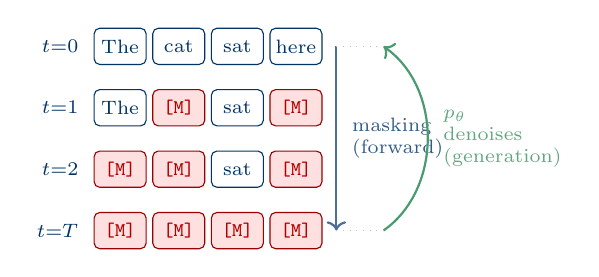
\begin{tikzpicture}[
    font=\scriptsize,
    token/.style={
      draw=navyblue, rounded corners=2pt,
      inner sep=2pt, minimum width=0.66cm, minimum height=0.46cm,
      fill=white, text=navyblue
    },
    mtoken/.style={
      draw=red!60!black, rounded corners=2pt,
      inner sep=2pt, minimum width=0.66cm, minimum height=0.46cm,
      fill=red!12, text=red!70!black
    },
    rlabel/.style={font=\scriptsize\bfseries, text=navyblue, anchor=east},
  ]
    %── FORWARD: masking goes down ──────────────────────────────────────
    \node[rlabel] (fl0) at (0,0)     {$t{=}0$};
    \node[token, right=2pt of fl0]  (f00) {The};
    \node[token, right=2pt of f00]   (f01) {cat};
    \node[token, right=2pt of f01]   (f02) {sat};
    \node[token, right=2pt of f02]   (f03) {here};

    \node[rlabel] (fl1) at (0,-0.78) {$t{=}1$};
    \node[token,  right=2pt of fl1]  (f10) {The};
    \node[mtoken, right=2pt of f10]   (f11) {\MASK};
    \node[token,  right=2pt of f11]   (f12) {sat};
    \node[mtoken, right=2pt of f12]   (f13) {\MASK};

    \node[rlabel] (fl2) at (0,-1.56) {$t{=}2$};
    \node[mtoken, right=2pt of fl2]  (f20) {\MASK};
    \node[mtoken, right=2pt of f20]   (f21) {\MASK};
    \node[token,  right=2pt of f21]   (f22) {sat};
    \node[mtoken, right=2pt of f22]   (f23) {\MASK};

    \node[rlabel] (fl3) at (0,-2.34) {$t{=}T$};
    \node[mtoken, right=2pt of fl3]  (f30) {\MASK};
    \node[mtoken, right=2pt of f30]   (f31) {\MASK};
    \node[mtoken, right=2pt of f31]   (f32) {\MASK};
    \node[mtoken, right=2pt of f32]   (f33) {\MASK};

    %── Masking arrow (down) ────────────────────────────────────────────
    \draw[->, thick, navyblue!70]
      ([xshift=5pt]f03.east) -- ([xshift=5pt]f33.east)
      node[midway, right=2pt, align=left, text=navyblue!80]
        {masking\\(forward)};

    %── Generation: curved arrow from t=T back to t=0 ──────────────────
    \draw[->, thick, gengreen!80, bend right=55]
      ([xshift=22pt]f33.east) to
      node[midway, right=2pt, align=left, font=\scriptsize, text=gengreen!70]
        {$p_\theta$\\denoises\\(generation)}
      ([xshift=22pt]f03.east);

    %── Dotted horizontal lines connecting the two arrows ───────────────
    \draw[gray!50, dotted]
      ([xshift=5pt]f03.east) -- ([xshift=22pt]f03.east);
    \draw[gray!50, dotted]
      ([xshift=5pt]f33.east) -- ([xshift=22pt]f33.east);

  \end{tikzpicture}
  \end{center}
\end{columns}

\end{frame}

%══════════════════════════════════════════════════════════════════════════════
%  SLIDE 3: HOW MDLMs WORK — TRAINING OBJECTIVE AND INFERENCE
%══════════════════════════════════════════════════════════════════════════════
\begin{frame}{How Masked Diffusion LLMs Work: Training and Inference}

\begin{columns}[T]
\column{0.52\textwidth}

  \textbf{Training objective}

  A transformer $\theta$ learns to reconstruct masked tokens from their context.
  The objective is the Evidence Lower BOund (ELBO):
  \[
    \mathcal{L}(\theta)
      = \mathbb{E}_{t,\,\mathbf{x}_t \sim q(\cdot|\mathbf{x}_0)}
        \bigl[\log p_\theta(\mathbf{x}_0 \mid \mathbf{x}_t)\bigr]
  \]
  This is a variational lower bound on the data log-likelihood.

  \medskip
  \textbf{Fine-tuning} on private data $\mathcal{D}_\text{train}$ continues
  this exact same ELBO objective on the new corpus.

  \medskip
  \textbf{Inference:} start from a fully masked sequence $[\MASK{}]^n$,
  then iteratively unmask tokens by sampling from $p_\theta$ until the
  sequence is fully recovered.

\column{0.44\textwidth}
  \begin{block}{ELBO gap after fine-tuning}
    Member texts have \textbf{lower} ELBO than non-members after fine-tuning.
    The model reconstructs them more accurately because it has seen them
    during training.

    \medskip
    This ELBO gap is the core membership signal we exploit.
  \end{block}

  \vspace{0.8em}
  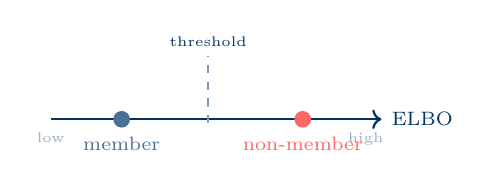
\begin{tikzpicture}[font=\scriptsize]
    \draw[->, thick, navyblue] (0,0) -- (4.2,0) node[right] {ELBO};
    \draw[navyblue!50, thick, dashed] (2.0, -0.05) -- (2.0, 0.8);
    \node[above, text=navyblue, font=\tiny] at (2.0,0.8) {threshold};
    \fill[navyblue!70] (0.9,0) circle (3pt) node[below=3pt] {member};
    \fill[red!60]      (3.2,0) circle (3pt) node[below=3pt] {non-member};
    \draw[navyblue!40] (0,-0.05) node[below]{\tiny low}
                       (4.0,-0.05) node[below]{\tiny high};
  \end{tikzpicture}
\end{columns}

\end{frame}

%══════════════════════════════════════════════════════════════════════════════
%  SLIDE 4: THE PRIVACY PROBLEM
%══════════════════════════════════════════════════════════════════════════════
\begin{frame}{The Privacy Problem}

\begin{columns}[T]
\column{0.50\textwidth}

  \textbf{Membership Inference Attack (MIA)}

  \medskip
  \textbf{Setup:} given white-box access to a fine-tuned MDLM and a text
  sample $x$, determine whether $x$ was in the fine-tuning data.

  \medskip
  \textbf{Prior work:} SAMA (Chen et al., 2026) introduced the first MIA
  designed for discrete diffusion models. It uses subset-aggregated loss
  differences and requires only grey-box access (output loss, no internals).

\column{0.46\textwidth}
  \begin{block}{Our approach}
    We extract a \textbf{46-dimensional feature vector} from the model's
    denoising trajectory and train a binary classifier.

    \medskip
    Features from 11 signal groups measured at 4 noise levels
    ($\alpha \in \{5\%,\,20\%,\,35\%,\,50\%\}$):

    \medskip
    {\footnotesize
    \begin{tabular}{@{}ll@{}}
      \toprule
      Signal group & What it captures \\
      \midrule
      ELBO trajectory   & loss at each $\alpha$ \\
      Entropy traj.     & prediction certainty \\
      Mask consistency  & multi-mask agreement \\
      Hidden-state norms & layer activations \\
      Attention patterns & cross-layer dynamics \\
      Cross-model cosine & fine-tuned vs base \\
      \bottomrule
    \end{tabular}
    }
  \end{block}
\end{columns}

\end{frame}

%══════════════════════════════════════════════════════════════════════════════
%  SLIDE 5: EXPERIMENT 1
%══════════════════════════════════════════════════════════════════════════════
\begin{frame}[shrink=5]{Experiment 1: Proof of Concept}

\begin{columns}[T]
\column{0.50\textwidth}

  \textbf{Data:} MIMIR GitHub — 300 members, 300 non-members.

  \medskip
  \textbf{Setup:} fine-tune \code{Qwen3-0.6B-MDLM} for 15 epochs to
  induce strong memorisation (loss: 3.86 $\to$ 1.59 nats).
  Extract the full \textbf{112-dimensional} feature vector using all 11 signal
  groups at $T=10$ timesteps plus the cross-model cosine similarity.

  \medskip
  \textbf{SAMA result:} AUC $= 0.369$ — below random chance. The attack
  is designed for moderate memorisation; heavy overfitting inverts its
  signal entirely. This revealed a design mismatch, not just an
  implementation bug.

  \medskip
  \textbf{Classifier result:} XGBoost on all 112 features achieves
  AUC $= 0.989$, TPR @ 1\% FPR $= 88.9\%$.

  \medskip
  White-box trajectory features are highly effective even in this
  small-sample setting where SAMA completely fails.

\column{0.46\textwidth}
  \begin{center}
  \includegraphics[width=\linewidth]{plots/sama_run1_vs_run2.pdf}
  \end{center}
  \vspace{-0.5em}
  \scriptsize
  SAMA AUC across Experiments 1 and 2, showing the design-mismatch issue
  and its resolution after adjusting the fine-tuning regime.
\end{columns}

\end{frame}

%══════════════════════════════════════════════════════════════════════════════
%  SLIDE 6: EXPERIMENT 2
%══════════════════════════════════════════════════════════════════════════════
\begin{frame}[shrink=5]{Experiment 2: Feature Refinement}

\begin{columns}[T]
\column{0.50\textwidth}

  \textbf{Same setting:} GitHub data, same model.

  \smallskip
  We reduced overfitting by using 5 epochs instead of 15, bringing SAMA
  back into its intended operating regime. We then refined the feature
  vector down to \textbf{46 dimensions} ($T=4$ timesteps instead of 10)
  while retaining all 11 signal groups:

  \begin{itemize}\setlength\itemsep{0.15em}
    \item ELBO values at $T=4$ noise levels
    \item Prediction entropy at each noise level
    \item Mask consistency across 8 random masking patterns
    \item Hidden-state norms and cross-layer cosine similarity
    \item Attention entropy, cross-layer attention (AttenMIA-inspired)
    \item Cross-model cosine (fine-tuned vs base model)
  \end{itemize}

  \smallskip
  The ELBO trajectory alone (4 numbers) outperforms SAMA on most
  metrics — pointing to it as the dominant signal.

\column{0.46\textwidth}
  \begin{center}
  
\includegraphics[width=\linewidth]{plots/tpr_all_methods.pdf}
  \end{center}
  \vspace{-0.5em}
  \scriptsize
  TPR across FPR thresholds on GitHub: our classifier separates
  cleanly from SAMA and the black-box baselines.
\end{columns}

\end{frame}

%══════════════════════════════════════════════════════════════════════════════
%  SLIDE 7: EXPERIMENT 3 SETUP
%══════════════════════════════════════════════════════════════════════════════
\begin{frame}{Experiment 3: Full Evaluation}

\begin{columns}[T]
\column{0.50\textwidth}

  \textbf{Scale-up:} 6 MIMIR domains, 12{,}000 samples.

  \medskip
  \begin{tabular}{@{}ll@{}}
    \toprule
    \textbf{Domain} & \textbf{Text type} \\
    \midrule
    ArXiv           & scientific papers \\
    GitHub          & source code \\
    HackerNews      & news and discussion \\
    PubMed Central  & biomedical abstracts \\
    Pile-CC         & CommonCrawl web text \\
    Wikipedia       & encyclopedic text \\
    \bottomrule
  \end{tabular}

  \medskip
  Per domain: fine-tune \code{Qwen3-0.6B-MDLM} on 1{,}000 members
  (5 epochs, lr $= 10^{-4}$), evaluate on 1{,}000 members and 1{,}000
  non-members using the 46-feature pipeline from Experiment 2.

\column{0.46\textwidth}
  \textbf{Attack classes compared:}

  \medskip
  \begin{block}{Black-box baselines}
    Loss, Zlib normalisation, Ratio (fine-tuned vs base model loss).
    Access: output loss only.
  \end{block}

  \begin{block}{Grey-box: SAMA (corrected)}
    Subset-aggregated masked-loss difference.
  \end{block}

  \begin{block}{White-box: our classifier}
    XGBoost and MLP trained on 46 trajectory features.
    5-fold cross-validation with 95\% CI on AUC.
  \end{block}
\end{columns}

\end{frame}

%══════════════════════════════════════════════════════════════════════════════
%  SLIDE 8: RESULTS
%══════════════════════════════════════════════════════════════════════════════
\begin{frame}{Results: AUC-ROC Across All Domains}

\begin{columns}[T]
\column{0.44\textwidth}
  \includegraphics[width=\linewidth]{plots/fig_roc_aggregate.pdf}
  \vspace{-0.3em}
  \scriptsize Mean ROC across 6 domains. Shaded band is $\pm$1 std.

\column{0.52\textwidth}
  {\small
  \begin{tabular}{@{}lccr@{}}
    \toprule
    \textbf{Domain} & \textbf{XGBoost} & \textbf{SAMA} & \textbf{Gap} \\
    \midrule
    Pile-CC      & 0.930 & 0.885 & +0.045 \\
    HackerNews   & 0.928 & 0.833 & +0.095 \\
    Wikipedia    & 0.892 & 0.823 & +0.069 \\
    ArXiv        & 0.877 & 0.783 & +0.094 \\
    PubMed       & 0.842 & 0.777 & +0.065 \\
    GitHub       & 0.801 & 0.795 & +0.006 \\
    \bottomrule
  \end{tabular}
  }

  \vspace{0.6em}
  \textbf{TPR at 1\% FPR:}
  \begin{itemize}
    \item XGBoost: \textbf{15–39\%} across domains
    \item SAMA: 3–10\%
    \item \textbf{4–8$\times$ improvement} at this threshold
  \end{itemize}

  \vspace{0.4em}
  GitHub is hardest: source code has high structural regularity across
  members and non-members, making the membership signal noisier despite
  having the largest ELBO gap of any domain.
\end{columns}

\end{frame}

%══════════════════════════════════════════════════════════════════════════════
%  SLIDE 9: ABLATION STUDY
%══════════════════════════════════════════════════════════════════════════════
\begin{frame}[shrink=5]{Ablation: What Drives Detection?}

\begin{columns}[T]
\column{0.50\textwidth}
  \includegraphics[width=\linewidth]{plots/fig_feature_ablation.pdf}
  \vspace{-0.3em}
  \scriptsize Leave-one-group-out AUC drop, averaged across 6 domains.
  Larger drop = group matters more.

\column{0.46\textwidth}

  Leave one feature group out, retrain, measure AUC drop.

  \smallskip
  {\small
  \begin{tabular}{@{}lr@{}}
    \toprule
    \textbf{Feature group} & \textbf{Mean AUC drop} \\
    \midrule
    ELBO trajectory      & $\mathbf{+0.142}$ \\
    Predictive entropy   & $+0.081$ \\
    Hidden-state norms   & $+0.012$ \\
    Mask consistency     & $+0.002$ \\
    Attention features   & $\approx 0$ \\
    \bottomrule
  \end{tabular}
  }

  \smallskip
  \begin{itemize}\setlength\itemsep{0.2em}
    \item ELBO trajectory dominates — removing it alone drops AUC by 0.142
    \item Prediction entropy adds a secondary but real signal (+0.081)
    \item Attention features are redundant once ELBO and entropy are present
    \item Just 8 features (ELBO + entropy, 4 each) capture most of the
      discriminative power
  \end{itemize}

  \smallskip
  Why is low-noise ELBO so informative? The next two slides explain.
\end{columns}

\end{frame}

%══════════════════════════════════════════════════════════════════════════════
%  SLIDE 10: THEORY — WEI ET AL. FRAMEWORK
%══════════════════════════════════════════════════════════════════════════════
\begin{frame}[shrink=2]{Privacy Theory: Wei et al.\ (2023)}

\begin{columns}[T]
\column{0.50\textwidth}

  Wei et al.\ derive per-instance differential privacy (pDP) guarantees
  for discrete denoising diffusion models.

  \medskip
  \textbf{Their transition:} uniform noise over vocabulary of size $K$:
  \[
    Q_t = \alpha_t I + (1 - \alpha_t) \cdot \frac{\mathbf{1}\mathbf{1}^\top}{K}
  \]
  Any token can become any other token with equal probability.

  \medskip
  \textbf{Per-instance DP (pDP):} measures privacy leakage specifically
  for one record $v^*$ given a training set of size $s+1$. The question:
  how much does the model's output shift when $v^*$ is included vs excluded?

\column{0.46\textwidth}
  \begin{block}{MDLM transition (absorbing)}
    MDLMs use:
    \[
      Q_t = \alpha_t I + (1 - \alpha_t)\,\mathbf{e}_{\MASK} \mathbf{1}^\top
    \]
    A token can only become \MASK, not any arbitrary vocabulary token.
    Once masked, it stays masked — this is the absorbing state.
  \end{block}

  \vspace{0.5em}
  The Wei et al.\ framework is the right tool to reason about MDLM
  privacy, but their bound was derived for the uniform case and does not
  transfer directly to the absorbing transition.
\end{columns}

\end{frame}

%══════════════════════════════════════════════════════════════════════════════
%  SLIDE 11: THEORY — THEOREM
%══════════════════════════════════════════════════════════════════════════════
\begin{frame}{Privacy Theory: The Bound}

\begin{columns}[T]
\column{0.50\textwidth}

  \textbf{Theorem 1 (Wei et al., simplified):}

  \[
    \delta(v^*,\varepsilon)
      \;\lesssim\;
      \underbrace{\bar{R}_t^{\,n-1}}_{\text{noise factor}}
      \;\cdot\;
      \underbrace{\frac{m}{s\,\varepsilon}}_{\text{data factor}}
  \]

  where $\bar{R}_t = \bar{\alpha}_t$ is the cumulative masking level,
  $n$ is sequence length, $m$ is generation length,
  and $s$ is the number of other training records.

  \medskip
  \textbf{What the noise factor means:}
  \begin{itemize}
    \item At \textbf{high noise} ($t \to T$): $\bar{\alpha}_t \to 0$, so
      $\bar{R}_t^{n-1} \to 0$. Leakage is near zero — masking hides the data.
    \item At \textbf{low noise} ($t \to 0$): $\bar{\alpha}_t \to 1$, so
      $\bar{R}_t^{n-1} \to 1$. Leakage reaches $O(m/s\varepsilon)$ — the
      model is close to the training data and membership leaks.
  \end{itemize}

\column{0.46\textwidth}

  \textbf{Why this connects to the ablation:}

  \medskip
  Our ELBO features are measured at low masking ratios
  ($\alpha \in \{5\%,\,20\%,\,35\%,\,50\%\}$).
  At these levels $\bar{\alpha}_t$ is close to 1, so the noise factor
  $\bar{R}_t^{n-1}$ is near its maximum.

  \medskip
  The theorem tells us this is exactly the regime of highest privacy
  leakage. Our features probe the model precisely where membership
  information is most exposed — which is why ELBO at low noise is the
  dominant signal.

  \smallskip
  \begin{alertblock}{The gap}
    Wei et al.\ assume uniform transitions. MDLMs use absorbing transitions.
    The bound does not yet apply directly.
  \end{alertblock}
\end{columns}

\end{frame}

%══════════════════════════════════════════════════════════════════════════════
%  SLIDE 12: FUTURE WORK
%══════════════════════════════════════════════════════════════════════════════
\begin{frame}[shrink=5]{Future Work}

\begin{columns}[T]
\column{0.48\textwidth}

  \begin{block}{Experiment 4 — LLaDA-8B}
    Apply the same pipeline to LLaDA-8B (8B parameters, 13$\times$ larger).
    Does greater capacity change the attack surface? Do larger models
    memorise more precisely, or generalise enough to hide individual records?
  \end{block}

  \vspace{0.3em}
  \begin{block}{Bound for Absorbing Transitions}
    Wei et al.\ use uniform noise:
    $Q_t = \alpha_t I + (1-\alpha_t)\tfrac{\mathbf{1}\mathbf{1}^\top}{K}$

    MDLMs use absorbing noise:
    $Q_t = \alpha_t I + (1-\alpha_t)\,\mathbf{e}_{\MASK}\mathbf{1}^\top$

    \smallskip
    Goal: derive the analogue of Theorem 1 for the absorbing case. Does
    concentrating noise on a single state give stronger or weaker privacy
    than spreading it uniformly?
  \end{block}

\column{0.48\textwidth}

  \textbf{Summary}

  \smallskip
  \begin{itemize}
    \setlength\itemsep{0.3em}
    \item White-box features substantially outperform SAMA and all
      black-box baselines across all 6 domains.
    \item The ELBO trajectory (4 numbers) drives most of the classifier's
      performance. Attention features add nothing.
    \item MDLMs are more privacy-vulnerable than prior work suggested.
    \item Wei et al.\ (2023) explain why: low-noise ELBO is exactly the
      regime of maximum privacy leakage.
  \end{itemize}

  \vspace{0.6em}
  \begin{center}
    \large\textbf{Thank you.}
  \end{center}
\end{columns}

\end{frame}

%══════════════════════════════════════════════════════════════════════════════
%  SLIDE 13: REFERENCES
%══════════════════════════════════════════════════════════════════════════════
\begin{frame}[allowframebreaks]{References}
  \scriptsize
  \begin{enumerate}
    \setlength\itemsep{0.5em}

    \item Y.~Chen, K.~Zhang, Y.~Du, E.~Stoppa, C.~Fleming, A.~Kundu,
      B.~Ribeiro, and N.~Li.
      \textbf{Membership Inference Attacks Against Fine-tuned Diffusion Language
      Models.}
      \textit{ICLR 2026.} arXiv:2601.20125.

    \item R.~Wei, E.~Kreacic, H.~Wang, H.~Yin, E.~Chien, V.\,K. Potluru,
      and P.~Li.
      \textbf{On the Inherent Privacy Properties of Discrete Denoising Diffusion
      Models.}
      \textit{arXiv:2310.15524}, 2023.

    \item P.~Zaree, M.\,A. Al~Mamun, Y.~Dong, I.~Alouani, and N.~Abu-Ghazaleh.
      \textbf{AttenMIA: LLM Membership Inference Attack through Attention
      Signals.}
      \textit{arXiv:2601.18110}, 2026.

    \item D.~Duan, A.~Suri, N.~Mireshghallah, T.~Le, W.~Shi, Y.~Zhu,
      T.~Shi, M.~Ryabinin, J.~Min, and Y.~Tsvetkov.
      \textbf{Do Membership Inference Attacks Work on Large Language Models?}
      \textit{arXiv:2402.07841}, 2024. (MIMIR benchmark)

  \end{enumerate}
\end{frame}

%─────────────────────────────────────────────────────────────────────────────
\end{document}
